
\documentclass[table,dvipsnames]{beamer}
\mode<presentation>{
	\usetheme{Madrid}
	\setbeamercolor{title}{fg=Black,bg=Blue!15}
	\setbeamercolor{frametitle}{fg=Black,bg=Blue!15}
	\setbeamercolor{block title}{fg=Black,bg=Blue!15}
	\setbeamercolor{block}{fg=Black,bg=Blue!10}
}

\usepackage{default}
\usepackage{graphicx}
\usepackage{booktabs}
\usepackage{xcolor}
\usepackage{multirow}

\title[STM32 Beginner Guide]{Pengenalan Multithreading dan interfacing STM32}
\author{}
\institute[Achmadi ST MT]{
	Institut Teknologi Sepuluh November  \\
	\vspace{10pt}
	FTITOS
	\vspace{10pt}
	CodeDirect
	\medskip
	\textit{}
}
\date{}

\begin{document}
	
	\section{Start}
	
	\begin{frame}
	\titlepage
	\end{frame}

	\section{STM32}
	\subsection{Chip STM32}
	\begin{frame}
		\frametitle{Produk Chip STM32}
		\begin{block}{}
			Chip STM32 adalah microcontroller yang diproduksi ST Microelectronic.
		\end{block}
	
		\begin{block}{}
			Menggunakan arsitektur 32-bit ARM Cortex M0/M3/M4.
		\end{block}
	
		\begin{block}{}
			Standar Industri, tersedia tools dan compiler/toolchain untuk development.
		\end{block}
		\begin{center}
			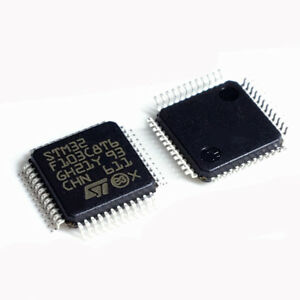
\includegraphics[width=150pt]{images/stm32f103c8}
		\end{center}
	\end{frame}

	\subsection{Board Discovery}
	\begin{frame}
		\frametitle{STM32 Discovery}
		\begin{block}{}
			ST menyediakan beberapa macam board untuk belajar pemula maupun pengembangan awal.
		\end{block}
		
		\begin{center}
			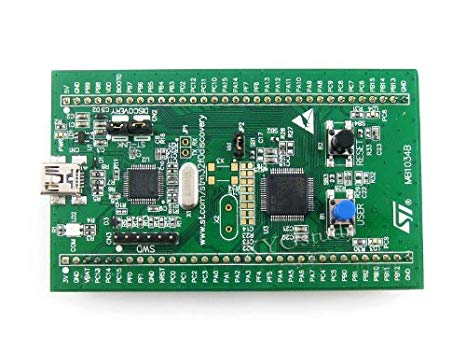
\includegraphics[width=150pt]{images/f0disco}
			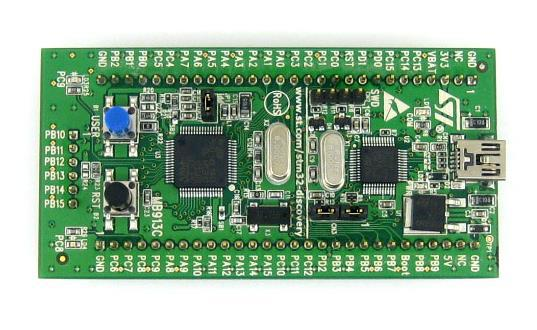
\includegraphics[width=150pt]{images/f1disco}
		\end{center}
	\end{frame}

	\begin{frame}
		\frametitle{STM32 Discovery}
		
		\begin{block}{}
			Tersedia board Discovery untuk seri STM32F0, STM32F1, STM32F2, STM32F3, dan STM32F4.
		\end{block}
		
		\begin{center}
			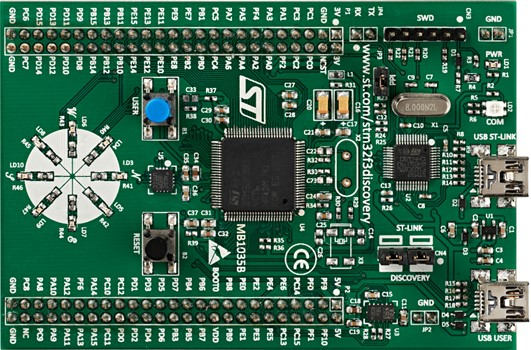
\includegraphics[width=125pt]{images/f3disco}
			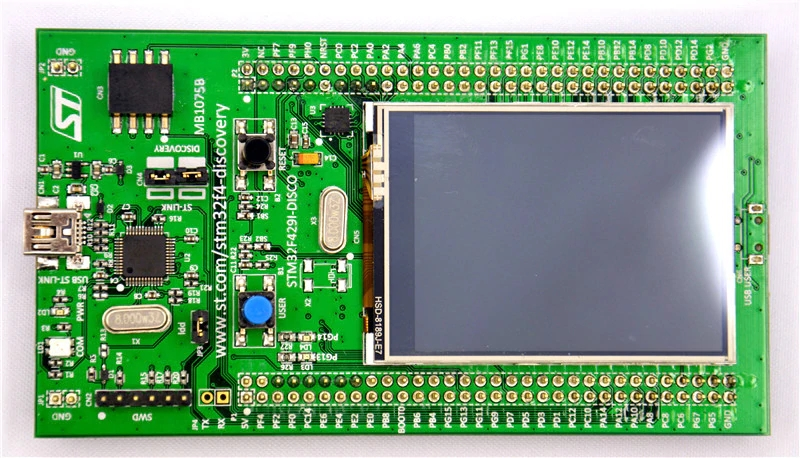
\includegraphics[width=150pt]{images/f4disco}
		\end{center}
	\end{frame}

	\subsection{Nucleo Discovery}
	\begin{frame}
		\frametitle{STM32 Nucleo}
		\begin{block}{}
			Selain Discovery, ST juga menyediakan board Nucleo yang memiliki pin-header layout
			kompatibel dengan Arduino.
		\end{block}
		
		\begin{center}
			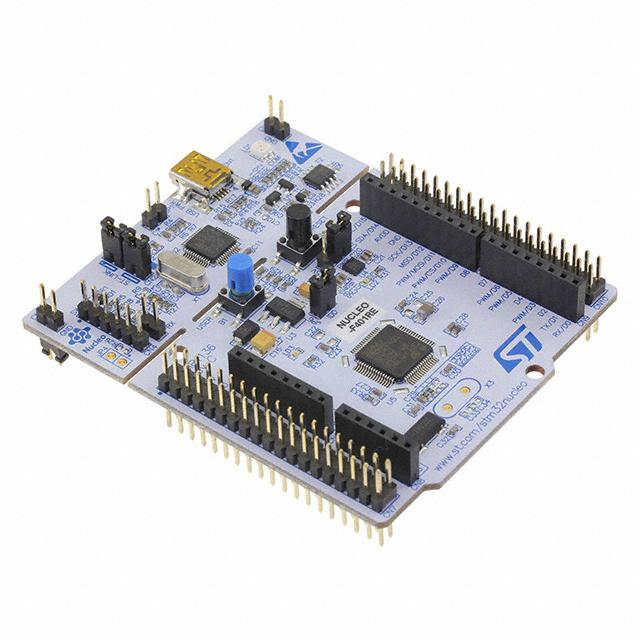
\includegraphics[width=200pt]{images/nucleo}
		\end{center}
	\end{frame}

	\subsection{Unofficial Board}
	\begin{frame}
		\frametitle{STM32 Nucleo}
		\begin{block}{}
			Selain Discovery dan Nucleo, tersedia juga board STM32 yang bukan dibuat oleh ST.
		\end{block}
		
		\begin{center}
			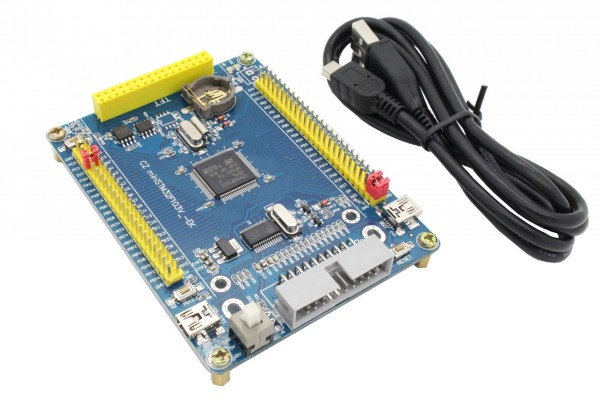
\includegraphics[width=150pt]{images/czmini}
			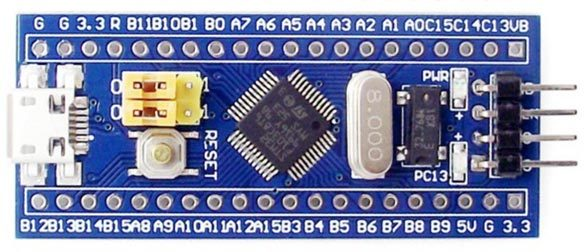
\includegraphics[width=150pt]{images/bluepill}
		\end{center}
	\end{frame}

\end{document}
